\documentclass{article}
\usepackage[utf8]{inputenc}
\usepackage{polski}
\usepackage[polish]{babel}
\usepackage{bbm}
\usepackage{graphicx}    
\usepackage{caption}
\usepackage{subcaption}
\usepackage{epstopdf}
\usepackage{amsmath}
\usepackage{amsthm}
\usepackage{hyperref}
\usepackage{url}
\usepackage{comment}
\newtheorem{defi}{Definicja}
\newtheorem{twr}{Twierdzenie}
\usepackage{listings}
\usepackage{float}


\author{Michał Martusewicz 282023}
\date{Wrocław, \today}
\title{\textbf{Interpolowanie krzywych funkcją sklejaną}  \\ Sprawozdanie do zadania P.2.12}

\begin{document}
\maketitle
\section{Wstęp}

Wybrane przeze mnie zadanie polega na interpolacji pewnych krzywych.
 W \S 2 wyjaśnię, czemu wybieram metodę krzywej parametrycznej.
 W \S 3 przedstawię interpolację wielomianem.
 W \S 4 pokażę algorytm obliczania okresowej funkcji sklejanej.
 W \S 5 pokażę jego zastosowanie na przykładzie.
 W \S 6 przedstawię funkcję odczytującą dane z pliku i powiem krótko o naturalnej funkcji sklejanej.
 W \S 7 przeanalizuję odchylenie funkcji sklejanych od pewnych funkcji bibliotecznych.
 W \S 8 podsumuję moje badania.
 

\section{Wybór metody}

W zadaniu podane były dwie możliwe metody tworzenia odpowiednich krzywych:
\\

 a) podzielić ciąg punktów na takie podciągi, żeby każdy z nich zawierał punkty leżące na wykresie pewnej funkcji;
uzyskać przybliżoną postać linii wzorcowej łącząc wykresy przybliżeń tych funkcji; \\
b) potraktować linię jako krzywą parametryczną $[x(t), y(t)]$, gdzie t jest parametrem przebiegającym przedział
$[1, n]$, tak więc $x_i = x(i)$, $y_i = y(i)$ dla $i = 1, 2, \ldots , n$; zrekonstruować funkcje $x(t), y(t)$ stosując interpolację.

Na początek wybrałem metodę a). W celu przetestowania tej metody narysowałem prosty rysunek $\Omega$.Oczywiście większości krzywych (w tym i mojej $\Omega$) nie da się przedstawić za pomocą jednej funkcji. Rysunek przybliżyłem więc za pomocą różnych funkcji: prostej, $\arccos$ i okręgu, odpowiednio przesuniętych i z dobranymi odpowiednimi współczynnikami, które następnie posklejałem. Otrzymałem kształt odpowiadający oryginałowi, przedstawiony jest on na rysunku nr \ref{omega}. Ze względu na czytelność sprawozdania nie będę tu szczegółowo przedstawiał programu rysującego tę Omegę, znajduje się on w pliku ''omega.jl''. 

Szybko jednak okazało się, że wybrana metoda nie zadziała dla dowolnej krzywej. Łatwo to można zauważyć próbując przybliżyć funkcjami uproszczony rysunek stołu (na rysunku nr \ref{stol}). Pionowych kresek nie przybliży żadna funkcja, ponieważ z definicji funkcji jednemu argumentowi można przyporządkować co najwyżej jedną wartość. Rozwiązaniem mogło by być stworzenie bardzo wielu funkcji których w dziedzinie znajduje się tylko jeden, ten sam argument, ale nie stworzylibyśmy w ten sposób linii ciągłej.

Z tego powodu w dalszej części sprawozdania rozważał będę tylko metodę b).

\begin{figure}[H]
    \centering
	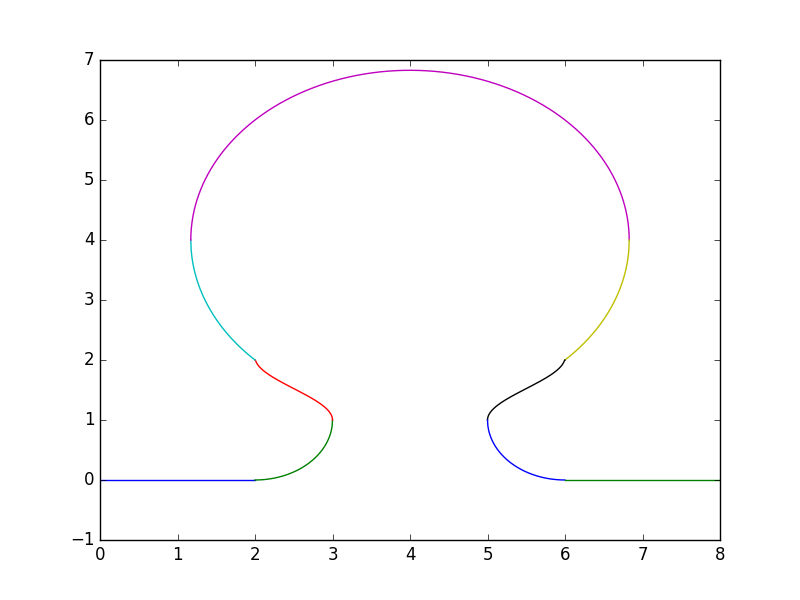
\includegraphics[width= 0.7 \textwidth]{omega.png}
    \caption{Przybliżenie rysunku $\Omega$ kolejno funkcjami: prostej, okręgu, $\arccos$, okręgu, $\arccos$, okręgu,prostej. }
 	\label{omega}
\end{figure}
\begin{figure}[H]
    \centering
	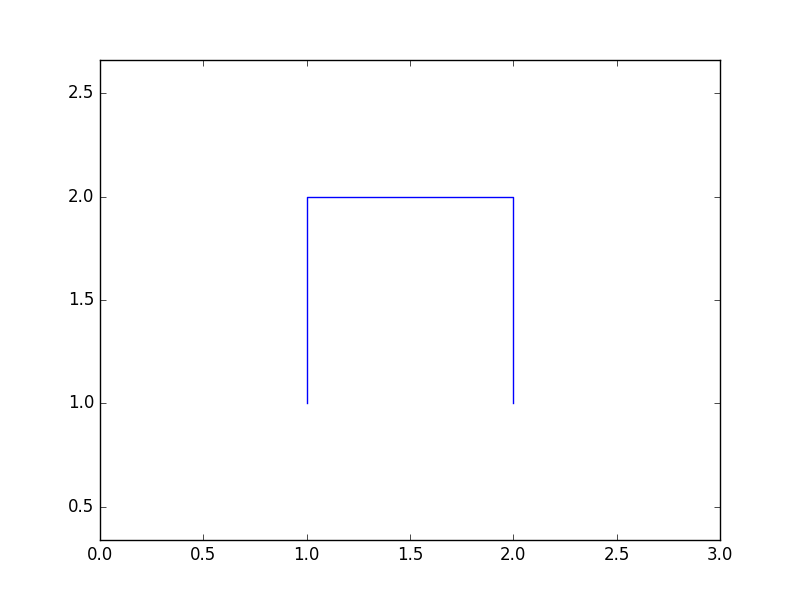
\includegraphics[width= 0.5 \textwidth]{stol.png}
    \caption{Rysunku stołu nie da się przybliżyć żadną funkcją, problemem są tu nogi.}
 	\label{stol}
\end{figure}

\section{Interpolacja wielomianowa}

W celu wyboru najlepszej metody narysowałem pewną krzywą i zebrałem z niej punkty znajdujące się w tabeli nr \ref{mrchw}. W zadaniu nie zdefiniowano konkretnej metody znajdowania funkcji interpolującej daną krzywą parametryczną, dlatego będę testował kolejne metody na tym właśnie rysunku.\\
\begin{table}[t]
\caption{Punkty z pewnej narysowanej krzywej}
\label{mrchw}
\begin{tabular}{|c|}
\hline
\begin{lstlisting}
(4.6,0.3)	(5.0,0.7)	(7.0,7.0)	(7.9,9.9)	
(8.0,10.3)	(7.7,10.7)	(7.0,11.5)	(7.1,12.3)	
(7.8,13.1)	(8.7,13.2)	(9.8,16.3)	(9.9,16.5)	
(9.6,16.5)	(6.1,16.5)	(6.7,16.9)	(7.7,16.7)	
(9.2,17.2)	(9,18.3)	(7.7,18.5)	(6.8,17.3)	
(5.7,16.7)	(6.4,17.4)	(5.5,18.7)	(4.6,17.4)	
(5.3,16.7)	(4.2,17.3)	(3.3,18.5)	(2,18.3)	
(1.8,17.2)	(3.3,16.7)	(4.3,16.9)	(4.9,16.5)	
(1.5,16.5)	(1.1,16.5)	(1.1,16.3)	(2.0,11.0)	
(4.2,0.7)	(4.6,0.3)
\end{lstlisting}\\
\hline
\end{tabular}
\end{table}


Pierwszym, najprostszym pomysłem jest interpolacja wielomianowa. Metodę tę zaprogramowałem następująco: najpierw funkcja wylicza za pomocą ilorazów różnicowych współczynniki i je tablicuje, a potem uogólnionym schematem Hornera wylicza wartości kolejnych $x(t)$ i $y(t)$ i zaznaczam je na wykresie.

Pewną trudnością było odpowiednie dobranie współczynnika $t$. Pierwszym wyborem były punkty równoodległe, jednak efekt był dalece nie zadowalający, co widać na rysunku \ref{r-w}. Niektóre wartości krzywej były nawet rzędu $10^14$, czego jednak ze względu na czytelność rysunku na niem nie ująłem. Łatwo wytłumaczyć niepowodzenie tej metody. Wiadomo, że przy równoodległych punktach wielomiany ,,wybuchają'' przy końcach przedziału, stąd tylko środek rysunku jest dość dobrze odwzorowany. 
\begin{figure}[H]
    \centering
	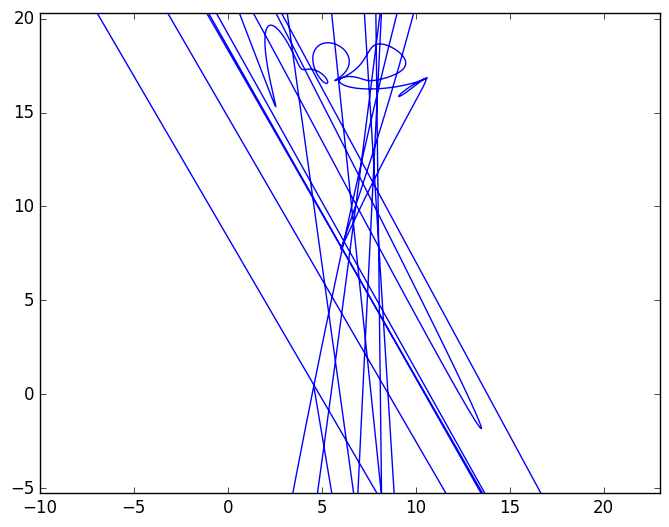
\includegraphics[width= 0.5 \textwidth]{rownoodlegle-wielomiany.png}
    \caption{Przybliżenie narysowanej krzywej wielomianem, dla równoodległych warości $t$.  }
 	\label{r-w}
\end{figure}
Kolejnym sposobem było wybranie kolejnych t w miejscach, w których znajdują się kolejne pierwiastki wielomianu Czebyszewa n-tego stopnia. Kolejne wartości zostały wyrażone zatem według wzoru: $ t_{i}=\cos \left({\frac  {2 * i-1}{2 * n}}* \pi \right)$, dla $i=1,2,\ldots ,n$. Wykres dla takich $t$ został przedstawiony na rysunku nr \ref{c-w}. Krzywa jest już znacząco lepiej przybliżona, przede wszystkim wszystkie wartości krzywej są rzędu mniejszego niż $10^2$ i nie ,,wybuchają'' przy końcach. Niestety odwzorowanie nie było w pełni satysfakcjonujące z dwóch powodów. Po pierwsze rysunek nie jest aż tak dobrze oddany, pewne nieprzecinające się w rzeczywistości linie przecinają się na wykresie. Po drugie krzywa podana była jako krzywa zamknięta, a wykres jest krzywą otwartą. Na niedokładność tej metody prawdopodobnie wpływa również pena niedokładność obliczeń komputerowych, choć wszystkie były wykonywane na BigFloatach przy wartości setprecision() ustawionej na co najmniej 300. To jednak pokazuje, że interpolacja wielomianem nie jest najlepszym pomysłem.
\begin{figure}[H]
    \centering
	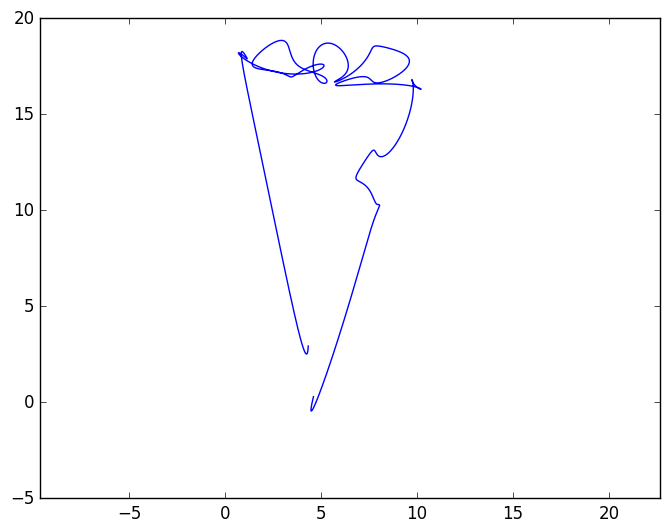
\includegraphics[width= 0.6 \textwidth]{welomian-czebyszew.png}
    \caption{}
 	\label{c-w}
\end{figure}

\section{Algorytm okresowej funkcji sklejanej}


\textbf{Twierdzenie}

Dla danej liczby naturalnej $n$, danych węzłów $x_0, x_1, \ldots , x_n$ $(a = x_0 < x_1 < \ldots < x_n = b)$
i danej funkcji f istnieje dokładnie jedna funkcja 
$\tilde{s} \in C^2 [a, b]$, zwana okresową funkcją
sklejaną interpolacyjną III stopnia, spełniająca następujące warunki:
\begin{enumerate}
\item w każdym z podprzedziałów $[x_{k-1} , x_k ] (k = 1, 2, \ldots, n)$ funkcja $\tilde{s}$ jest identyczna z pewnym wielomianem stopnia co najwyżej trzeciego;
\item $\tilde{s}(x_k ) = f(x_k ) (k = 0, 1, \ldots , n)$;
\item $\tilde{s}^{(i)} (a + 0) = \tilde{s}^{(i)} (b - 0)$ $(i = 0, 1, 2)$.
\end{enumerate}

(Łatwo zauważyć, że warunek 3. pociąga za sobą równość $f(x_n ) = f(x_0 )$). W każdym z przedziałów
$[x_{k-1} , x_k ]$ $(k = 1, 2, \ldots , n)$ jest
\begin{eqnarray*}
\tilde{s}(x) &=&  h_k^{-1} \Bigg\{ \frac{1}{6}M_{k-1} (x_k - x)^3 +\frac{1}{6} M_k (x - x_{k-1})^3 
\\ 
&+& \left[ (x_{k-1} ) - \frac{1}{6} M_{k-1} h_k^2 \right] (x_k - x) + \left[f(x_k) -\frac{1}{6} M_k h_k^2  \right] (x - x_{k-1} ) \Bigg\}
\end{eqnarray*}


Wartości $M_k := \tilde{s}'' (x_k)$ $(k = 0, 1, \ldots , n)$ spełniają układ
$$
\lambda_k M_{k-1} + 2M_k + (1 - \lambda_k )M_{k+1} = d_k\qquad (k = 1, 2, \ldots, n)
$$


gdzie $M_{n+1} := M_1 , M_0 = M_n$ oraz

$$
d_k :=\frac{6}{h_k + h_{k+1}}\left[ \frac{f(x_{k+1} ) - f(x_k)}{h_{k+1}} - \frac{ f(x_k ) - f(x_{k-1} )}{h_k}\right]
\lambda_k := h_k /(h_k + h_{k+1} )
(k = 1, 2, \ldots , n),
$$
gdzie z kolei $f(x_{n+1} ) := f(x_1 )$ i $h_{n+1} := h_1 $.
Zauważmy, że ten układ równań można przedstawić za pomocą następującej macierzy: \\

$
\begin{bmatrix} 
2&1-\lambda_1&0&0&\ldots&\lambda_1\\ 
\lambda_2&2&1-\lambda_2&0&\ldots&0\\ 
0&\lambda_3&2&1-\lambda_3&\ldots&0\\ 
\vdots & \vdots&\vdots&\ddots&\vdots&\vdots\\
0&\ldots&0&\lambda_{n-1}&2&1-\lambda_{n-1}\\
1-\lambda_n&0&\ldots&0  & \lambda_n&2 
\end{bmatrix}
$
$ \begin{bmatrix} 
M_1\\
M_2\\
M_3\\
\vdots \\
M_{n-1}\\
M_n
\end{bmatrix}
=$
$ \begin{bmatrix} 
d_1\\
d_2\\
d_3\\
\vdots \\
d_{n-1}\\
d_n
\end{bmatrix}
$\\

Algorytm ich rozwiązywania jest de facto rozwiązywaniem za pomocą eliminacji Gausa i jest lekko zmodyfikowaną wersją dla naturalnej funkcji sklejanej.
Algorytm ten przedstawia się następująco:

Obliczamy pomocnicze wielkości $p_1 , p_2 , \ldots , p_{n-1} , q_0 , q_1 , \ldots , q_{n-1} , u_0 , u_1 , \ldots , u_{n-1}
$ i $s_0 , s_1 , \ldots , s_{n-1} $ w następujący sposób rekurencyjny:\\

$q_0 := u_0 := 0,\quad s_0 := 1$,\\
dla $k=1,2,\ldots,n-1$ :
\begin{eqnarray*}
p_k &:=& \lambda_k q_{k-1} + 2,\\
q_k &:=& (\lambda_k - 1)/p_k ,\\
s_k &:=& -\lambda_k s_{k-1} /p_k ,\\
u_k &:=& (d_k - \lambda_k u_{k-1} )/p_k\\
\end{eqnarray*}
Zauważmy, że n - 1 początkowych równań naszego układu można zapisać jako
$M_k = q_k M_{k+1} + s_k M_n + u_k$
dla
$k = 1, 2, \ldots , n-1$
\\
Następnie definiujemy $t_0 , t_1 , \ldots , t_n$ i $v_0 , v_1 , \ldots , v_n$ za pomocą wzorów\\

$t_n := 1,\quad v_n := 0,$\\

dla $k = n-1, n-2, \ldots , 1$:

\begin{eqnarray*}
t_k &:=& q_k t_{k+1} + s_k ,\\
v_k &:=& q_k v_{k+1} + u_k
\end{eqnarray*}

Wówczas\\
$M_n = [d_n - (1 - \lambda_n )v_1 - \lambda_n v_{n-1} ]/[2 + (1 - \lambda_n )t_1 + \lambda_n t_{n-1} ]$,\\
$M_k = v_k + t_k M_n$
dla
$k = 1, 2, \ldots , n - 1$.\\
(\cite{bib1})
\section{Użycie okresowej funkcji sklejanej}

Zastosowałem powyższy algorytm do wyliczenia dwóch funkcji $\tilde{s}_x(t)$ i $\tilde{s}_y(t)$ składających się na krzywą parametryczną. Początkowo zastosowałem równoodległe t (rysunek \ref{r-o}. Jest to jednak niezbyt dobre rozwiązanie, gdyż odległości między punktami są znacząco różne. Ponadto powstają różne zakłamania, pętle i ''dziubki''.

\begin{figure}[H]
    \centering
	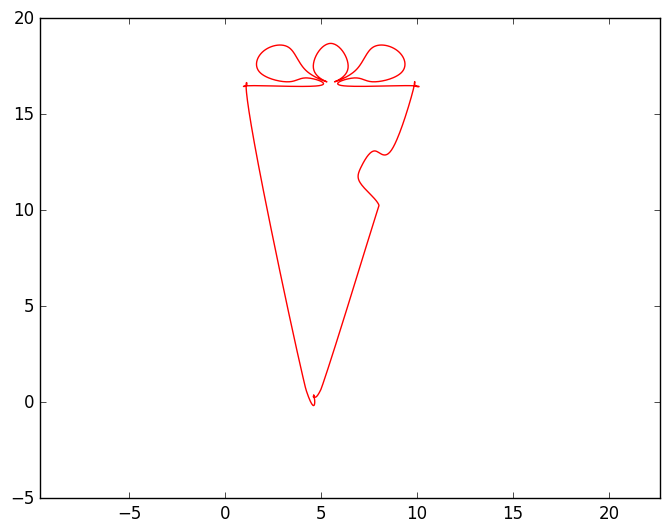
\includegraphics[width= 0.5 \textwidth]{okr-r.png}
    \caption{Okresowa funkcja sklejana dla równoodległych t }
 	\label{r-o}
\end{figure}

Postanowiłem zatem użyć tutaj twierdzenia Pitagorasa, wyliczając kolejne t według wzoru:
$t_i=t_{i-1}+\sqrt[2]{(x_i-x_{i-1})^2+(y_i-y_{i-1})^2}$,dla $i=1,2,\ldots,n$, przy czym $t_0=0$.
Jest to w przybliżony sposób wyliczona długość łuku pomiędzy kolejnymi punktami.
Dało to doskonałe efekty, co widać na rysunku numer \ref{p-o}. 
Ponadto użyłem tej funkcji do zinterpolowania tajemniczej krzywej z zadania \textbf{P2.11}. Efekt widoczny jest na rysunku numer \ref{polska}
\begin{figure}[H]
    \centering
	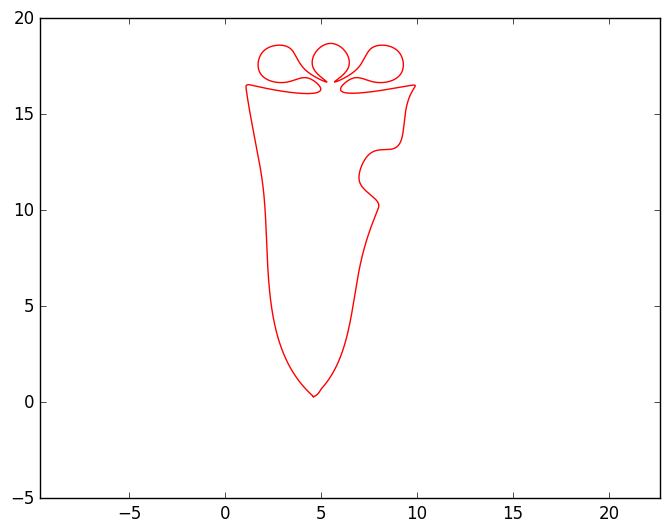
\includegraphics[width= 1 \textwidth]{okr-pit.png}
    \caption{Okresowa funkcja sklejana dla t określonych za pomocą odległości pomiędzy kolejnymi punktami. }
 	\label{p-o}
\end{figure}
\begin{figure}[H]
    \centering
	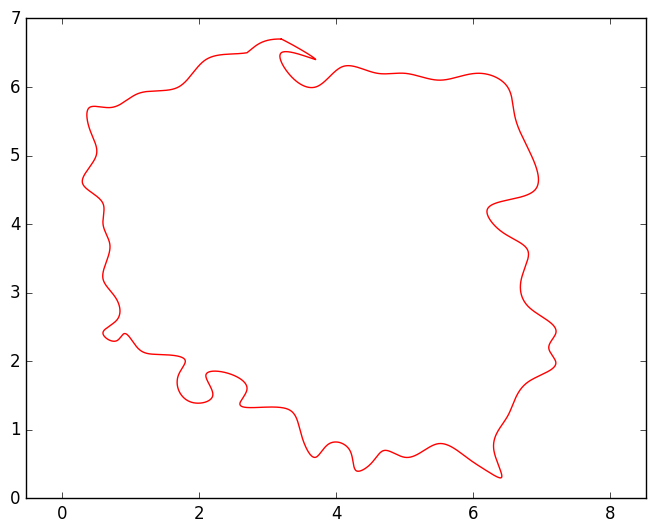
\includegraphics[width= 0.5 \textwidth]{polska.png}
    \caption{Okresowa funkcja sklejana dla t określonych za pomocą odległości pomiędzy kolejnymi punktami. }
 	\label{polska}
\end{figure}
\section{Odczytywanie punktów z pliku i naturalna funkcja sklejana}

Częścią zadania było również napisanie programu było zaimplementowanie funkcji umożliwiającej interpolowanie plików zawartych w osobnym pliku. Zrealizowałem to za pomocą funkcji interpol($\epsilon$, czyZpliku,nazwa,sposob,typ),   gdzie: \\
\begin{itemize}
\item $\epsilon$ to odległość pomiędzy kolejnymi punktami gotowej krzywej sklejanej, \\
\item czyZpliku przyjmuje wartość 1 (odczyt z pliku) lub 0 (wybór zaimplementowanej funkcji matematycznej); \\
\item nazwa to nazwa pliku (gdy czyZpliku=1) lub żądanej funkcji matematycznej (w przeciwnym przypadku);\\
\item sposob to sposób tworzenia t (''pitagoras'',''równoodległe'',''czebyszew'');\\
\item typ to typ funkcji (''okresowa'',''naturalna'',''wielomian'').\\
\end{itemize}
Funkcja zwraca krotkę (X,Y), gdzie X i Y są gotowymi tablicami z argumentami i odpowiadającymi im wartościami.
Format punktów w pliku musi być następujący:
$(x_0,y_0)<tab>(x_1,y_1)<tab>\ldots<tab>(x_n,y_n) $, gdzie $<tab>$ to znak tabulatora. W folderze prog załączone są przykładowe pliki: ''marchewka.pkt'' i ''polska.pkt''.

Ponieważ nie każda krzywa jest krzywą zamkniętą, zaimplementowałem również naturalną funkcję sklejaną. naturalna funkcja sklejana różni się od okresowej tylko tym, że w naturalnej na krańcach przedziałów druga pochodna jest równa zero, zaś w okresowej pierwsza i druga pochodna na krańcach przedziału równają się sobie. Algorytm obliczania funkcji okresowej jest ogólnie znany, dość prosty i podobny do algorytmu okresowej funkcji \cite{bib1}. Ponieważ szczęśliwie mój rysunek zaczyna się w odpowiednim miejscu, dlatego też 
naturalna funkcja sklejana interpoluje ją właściwie, co widać na rysunku numer \ref{p-n}.

\begin{figure}[H]
    \centering
	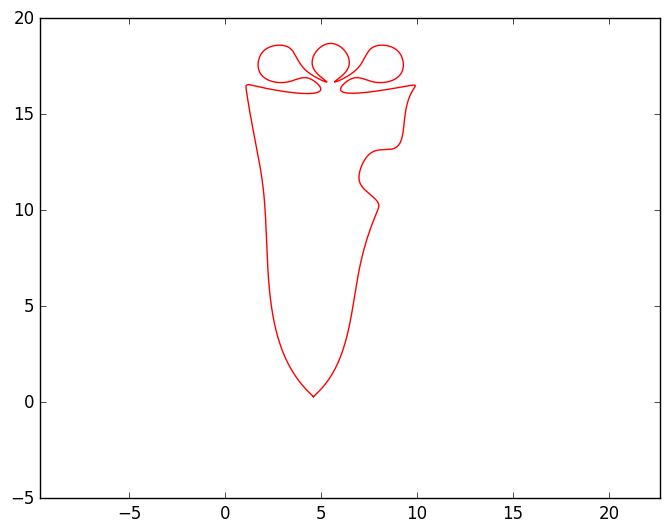
\includegraphics[width= 0.5 \textwidth]{nat-mrchw.png}
    \caption{Naturalna funkcja sklejana dla t określonych za pomocą odległości pomiędzy kolejnymi punktami. }
 	\label{p-n}
\end{figure}
\section{Analiza błędów} 

Postanowiłem sprawdzić dokładność interpolowanej krzywej na kilku przykładach.
Pierwszym wyborem był zwykły okrąg o promieniu 1. Dla takiej krzywej $x(t)=\cos t$, $y(t)=\sin t$.
Na rysunku numer \ref{okr} zostały nałożone na siebie wykresy funkcji sklejanej i funkcji bibliotecznych. Została również przedstawiona krzywa błędu, dla wygody przedstawiona w postaci $e(x)=\frac{-1}{16}*\log_{10}|f(x)-\tilde{s}(x)|$.
Jak widać krzywa błędu jest dość symetryczna (niesymetryczności wynikają zapewne z zaokrągleń i zbyt małej dokładności). Można zauważyć, że funkcja najdokładniejsza jest w okolicach zera i jeden, im dalej od zera, tym większy błąd. Jednak nawet w -1, gdzie błąd jest największy, nie przekracza on $10^{-2}$ co jest i tak jest nie do odróżnienia na rysunku. Stosując gęstsze próbkowanie i większą precyzję otrzymujemy lepsze przybliżenie, jednak program ma dość dużą złożoność obliczeniową i każde zwiększenie precyzji znacząco wydłuża czas obliczeń.
\begin{figure}[H]
    \centering
	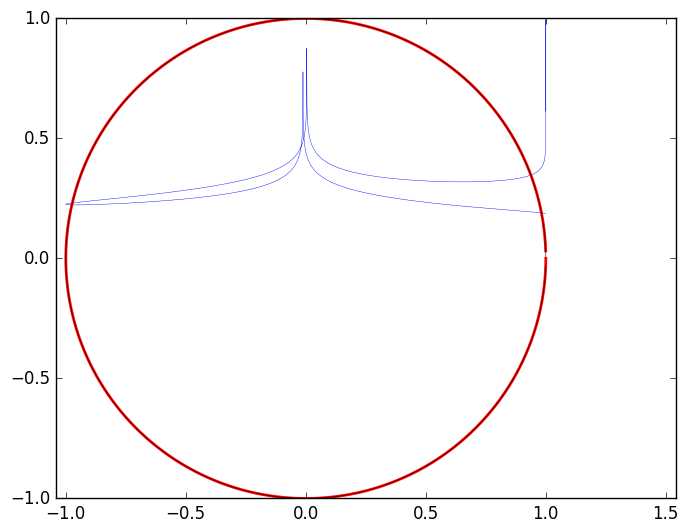
\includegraphics[width= 0.5 \textwidth]{okrag.png}
    \caption{Okrąg. Czerwona linia to wykres okresowej krzywej sklejanej, czarna to krzywa parametryczna korzystająca z funkcji bibliotecznych, a niebieska to $-1/8 \log_{10}(|\tilde{s}(x)-f(x)|) $ }
 	\label{okr}
\end{figure}

Jako inny przykład postanowiłem wybrać funkcję $f(x)=\sin x$ ze względu na to, że jest bardzo różna od funkcji wielomianowych. Interpolowałem ją naturalną funkcją sklejaną.
Efekt jest przedstawiony na rysunku numer \ref{sin}. Łatwo zauważyć, że generalnie błąd zawiera się w przedziale $[10^{-16},10^{-8}]$

\begin{figure}[H]
    \centering
	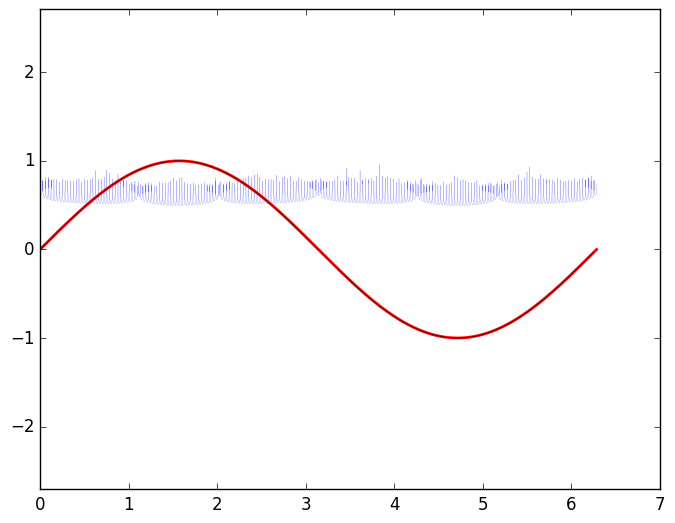
\includegraphics[width= 0.8 \textwidth]{sin.png}
    \caption{$f(x)=\sin(x)$. Czerwona linia to wykres naturalnej krzywej sklejanej, czarna to krzywa parametryczna korzystająca z funkcji bibliotecznych, a niebieska to $-1/16 \log_{10}(|s(x)-f(x)|) $}
 	\label{sin}
\end{figure}
\section{Wnioski}

Jest wiele różnych sposobów przybliżania krzywych. Nie każdą funkcję da się przybliżyć składanymi funkcjami, dlatego bardziej wartą uwagi wydaje się metoda krzywych parametrycznych. Do tego sposób przybliżenia tych krzywych również ma znaczenie. Najmniej dokładna jest interpolacja jednym wielomianem każdej krzywej, przy równoodległym parametrze t, wynika to z charakterystyki wielomianów, które "wybuchają" przy końcowych punktach. Gdy wybierzemy t jako kolejne zera wielomianu Czebyszewa n-tego stopnia, sytuacja znacząco poprawia się, jednak odwzorowanie dalej jest mocno niedokładne. Znacząco lepsza jest funkcja sklejana (zarówno naturalna, jak i okresowa), jednak przy równoodległym t mogą powstawać zaburzenia. Odległości pomiędzy punktami które interpolujemy zazwyczaj nie są równe, stąd lepszym rozwiązaniem jest przybliżenie tych odległości za pomocą twierdzenia Pitagorasa. Taka metoda jest już wystarczająco dokładna, co pokazują przykłady. Na dokładność możemy wpływać poprzez zwiększenie próbkowania krzywej, lub zwiększenie precyzji BigFloatów, jednak złożoność obliczeniowa metody jest znacząca, stąd czas dokładniejszych obliczeń jest dużo dłuższy.   
\begin{thebibliography}{9}
	\itemsep2pt
	    \bibitem{bib3} David Kincaid, Ward Cheney. Analiza numeryczna 

   \bibitem{bib5} A. Bjorck G. Dahlquist - Metody numeryczne (przekład S. Paszkowski, wydanie drugie, Warszawa 1987)
   \bibitem{bib1} S.Lewanowicz Analiza numeryczna, wykład 5
    
		
\end{thebibliography}

\end{document}

\end{document}